\documentclass{standalone}
\usepackage{tikz}
\usepackage{bm}
\begin{document}
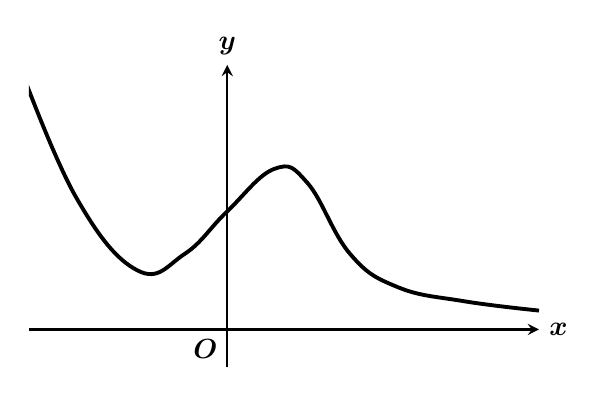
\begin{tikzpicture}[>=stealth, scale=0.6, font=\bfseries]
  % From unit2a/6-B.png: not exponential; local min left of the y-axis, local max right of it, then decays toward 0
  \draw[->, thick] (-4.2,0) -- (6.6,0) node[right] {$\bm{x}$};
  \draw[->, thick] (0,-0.8) -- (0,5.6) node[above] {$\bm{y}$};
  \node[below left] at (0,0) {$\bm{O}$};
  \begin{scope}
    \clip (-4.2,-0.8) rectangle (6.6,5.6);
    \draw[line width=1.4pt] plot[smooth, tension=0.7] coordinates {(-4.4,5.6) (-3.2,2.8) (-1.9,1.25) (-0.9,1.6) (0,2.5) (1.0,3.4) (1.7,3.1) (2.6,1.6) (3.6,0.9) (5,0.6) (6.6,0.4)};
  \end{scope}
\end{tikzpicture}
\end{document}
